% Created by tikzDevice version 0.10.1 on 2016-12-20 21:39:39
% !TEX encoding = UTF-8 Unicode
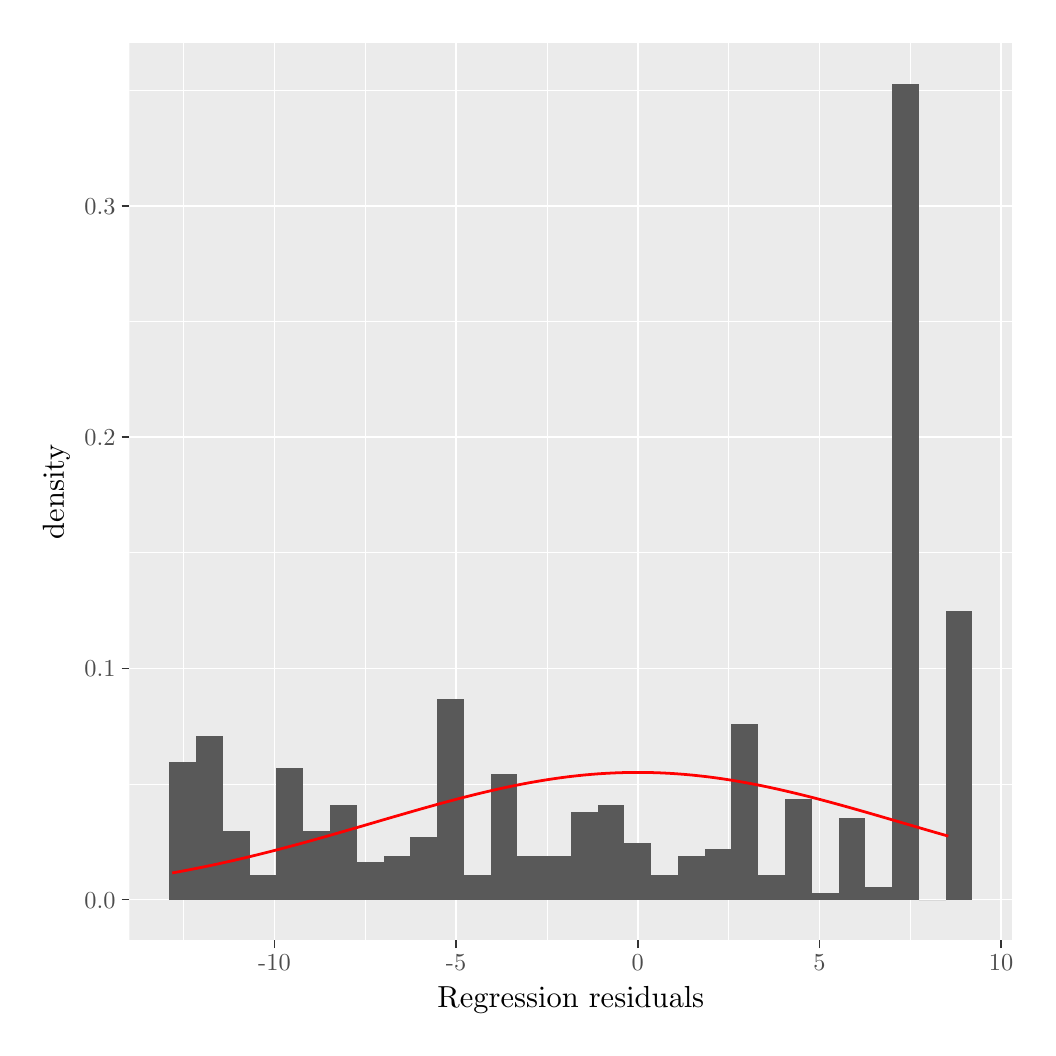
\begin{tikzpicture}[x=1pt,y=1pt]
\definecolor{fillColor}{RGB}{255,255,255}
\path[use as bounding box,fill=fillColor,fill opacity=0.00] (0,0) rectangle (361.35,361.35);
\begin{scope}
\path[clip] (  0.00,  0.00) rectangle (361.35,361.35);
\definecolor{drawColor}{RGB}{255,255,255}
\definecolor{fillColor}{RGB}{255,255,255}

\path[draw=drawColor,line width= 0.6pt,line join=round,line cap=round,fill=fillColor] (  0.00,  0.00) rectangle (361.35,361.35);
\end{scope}
\begin{scope}
\path[clip] ( 36.71, 31.53) rectangle (355.85,355.85);
\definecolor{fillColor}{gray}{0.92}

\path[fill=fillColor] ( 36.71, 31.53) rectangle (355.85,355.85);
\definecolor{drawColor}{RGB}{255,255,255}

\path[draw=drawColor,line width= 0.3pt,line join=round] ( 36.71, 88.04) --
	(355.85, 88.04);

\path[draw=drawColor,line width= 0.3pt,line join=round] ( 36.71,171.58) --
	(355.85,171.58);

\path[draw=drawColor,line width= 0.3pt,line join=round] ( 36.71,255.11) --
	(355.85,255.11);

\path[draw=drawColor,line width= 0.3pt,line join=round] ( 36.71,338.65) --
	(355.85,338.65);

\path[draw=drawColor,line width= 0.3pt,line join=round] ( 56.36, 31.53) --
	( 56.36,355.85);

\path[draw=drawColor,line width= 0.3pt,line join=round] (122.00, 31.53) --
	(122.00,355.85);

\path[draw=drawColor,line width= 0.3pt,line join=round] (187.64, 31.53) --
	(187.64,355.85);

\path[draw=drawColor,line width= 0.3pt,line join=round] (253.28, 31.53) --
	(253.28,355.85);

\path[draw=drawColor,line width= 0.3pt,line join=round] (318.92, 31.53) --
	(318.92,355.85);

\path[draw=drawColor,line width= 0.6pt,line join=round] ( 36.71, 46.27) --
	(355.85, 46.27);

\path[draw=drawColor,line width= 0.6pt,line join=round] ( 36.71,129.81) --
	(355.85,129.81);

\path[draw=drawColor,line width= 0.6pt,line join=round] ( 36.71,213.35) --
	(355.85,213.35);

\path[draw=drawColor,line width= 0.6pt,line join=round] ( 36.71,296.88) --
	(355.85,296.88);

\path[draw=drawColor,line width= 0.6pt,line join=round] ( 89.18, 31.53) --
	( 89.18,355.85);

\path[draw=drawColor,line width= 0.6pt,line join=round] (154.82, 31.53) --
	(154.82,355.85);

\path[draw=drawColor,line width= 0.6pt,line join=round] (220.46, 31.53) --
	(220.46,355.85);

\path[draw=drawColor,line width= 0.6pt,line join=round] (286.10, 31.53) --
	(286.10,355.85);

\path[draw=drawColor,line width= 0.6pt,line join=round] (351.74, 31.53) --
	(351.74,355.85);
\definecolor{fillColor}{gray}{0.35}

\path[fill=fillColor] ( 51.22, 46.27) rectangle ( 60.89, 96.17);

\path[fill=fillColor] ( 60.89, 46.27) rectangle ( 70.56,105.24);

\path[fill=fillColor] ( 70.56, 46.27) rectangle ( 80.23, 71.22);

\path[fill=fillColor] ( 80.23, 46.27) rectangle ( 89.90, 55.34);

\path[fill=fillColor] ( 89.90, 46.27) rectangle ( 99.57, 93.90);

\path[fill=fillColor] ( 99.57, 46.27) rectangle (109.24, 71.22);

\path[fill=fillColor] (109.24, 46.27) rectangle (118.91, 80.29);

\path[fill=fillColor] (118.91, 46.27) rectangle (128.58, 59.88);

\path[fill=fillColor] (128.58, 46.27) rectangle (138.26, 62.15);

\path[fill=fillColor] (138.26, 46.27) rectangle (147.93, 68.95);

\path[fill=fillColor] (147.93, 46.27) rectangle (157.60,118.85);

\path[fill=fillColor] (157.60, 46.27) rectangle (167.27, 55.34);

\path[fill=fillColor] (167.27, 46.27) rectangle (176.94, 91.63);

\path[fill=fillColor] (176.94, 46.27) rectangle (186.61, 62.15);

\path[fill=fillColor] (186.61, 46.27) rectangle (196.28, 62.15);

\path[fill=fillColor] (196.28, 46.27) rectangle (205.95, 78.02);

\path[fill=fillColor] (205.95, 46.27) rectangle (215.62, 80.29);

\path[fill=fillColor] (215.62, 46.27) rectangle (225.29, 66.68);

\path[fill=fillColor] (225.29, 46.27) rectangle (234.96, 55.34);

\path[fill=fillColor] (234.96, 46.27) rectangle (244.64, 62.15);

\path[fill=fillColor] (244.64, 46.27) rectangle (254.31, 64.42);

\path[fill=fillColor] (254.31, 46.27) rectangle (263.98,109.78);

\path[fill=fillColor] (263.98, 46.27) rectangle (273.65, 55.34);

\path[fill=fillColor] (273.65, 46.27) rectangle (283.32, 82.56);

\path[fill=fillColor] (283.32, 46.27) rectangle (292.99, 48.54);

\path[fill=fillColor] (292.99, 46.27) rectangle (302.66, 75.76);

\path[fill=fillColor] (302.66, 46.27) rectangle (312.33, 50.81);

\path[fill=fillColor] (312.33, 46.27) rectangle (322.00,341.11);

\path[fill=fillColor] (322.00, 46.27) rectangle (331.67, 46.27);

\path[fill=fillColor] (331.67, 46.27) rectangle (341.34,150.60);
\definecolor{drawColor}{RGB}{255,0,0}

\path[draw=drawColor,line width= 1.0pt,line join=round] ( 52.23, 55.91) --
	( 55.03, 56.42) --
	( 57.84, 56.95) --
	( 60.64, 57.50) --
	( 63.45, 58.06) --
	( 66.25, 58.64) --
	( 69.06, 59.24) --
	( 71.86, 59.86) --
	( 74.67, 60.49) --
	( 77.47, 61.14) --
	( 80.27, 61.81) --
	( 83.08, 62.49) --
	( 85.88, 63.19) --
	( 88.69, 63.90) --
	( 91.49, 64.63) --
	( 94.30, 65.37) --
	( 97.10, 66.12) --
	( 99.91, 66.88) --
	(102.71, 67.66) --
	(105.52, 68.44) --
	(108.32, 69.23) --
	(111.12, 70.04) --
	(113.93, 70.84) --
	(116.73, 71.66) --
	(119.54, 72.47) --
	(122.34, 73.29) --
	(125.15, 74.11) --
	(127.95, 74.94) --
	(130.76, 75.76) --
	(133.56, 76.57) --
	(136.37, 77.38) --
	(139.17, 78.19) --
	(141.97, 78.99) --
	(144.78, 79.78) --
	(147.58, 80.56) --
	(150.39, 81.33) --
	(153.19, 82.08) --
	(156.00, 82.82) --
	(158.80, 83.54) --
	(161.61, 84.24) --
	(164.41, 84.92) --
	(167.22, 85.58) --
	(170.02, 86.22) --
	(172.82, 86.83) --
	(175.63, 87.41) --
	(178.43, 87.97) --
	(181.24, 88.50) --
	(184.04, 88.99) --
	(186.85, 89.46) --
	(189.65, 89.89) --
	(192.46, 90.29) --
	(195.26, 90.66) --
	(198.07, 90.98) --
	(200.87, 91.28) --
	(203.67, 91.53) --
	(206.48, 91.75) --
	(209.28, 91.92) --
	(212.09, 92.06) --
	(214.89, 92.16) --
	(217.70, 92.22) --
	(220.50, 92.24) --
	(223.31, 92.22) --
	(226.11, 92.16) --
	(228.92, 92.06) --
	(231.72, 91.92) --
	(234.52, 91.74) --
	(237.33, 91.52) --
	(240.13, 91.27) --
	(242.94, 90.97) --
	(245.74, 90.65) --
	(248.55, 90.28) --
	(251.35, 89.88) --
	(254.16, 89.45) --
	(256.96, 88.98) --
	(259.77, 88.48) --
	(262.57, 87.95) --
	(265.37, 87.40) --
	(268.18, 86.81) --
	(270.98, 86.20) --
	(273.79, 85.56) --
	(276.59, 84.90) --
	(279.40, 84.22) --
	(282.20, 83.52) --
	(285.01, 82.80) --
	(287.81, 82.06) --
	(290.62, 81.30) --
	(293.42, 80.54) --
	(296.22, 79.76) --
	(299.03, 78.97) --
	(301.83, 78.17) --
	(304.64, 77.36) --
	(307.44, 76.55) --
	(310.25, 75.73) --
	(313.05, 74.91) --
	(315.86, 74.09) --
	(318.66, 73.27) --
	(321.47, 72.45) --
	(324.27, 71.63) --
	(327.07, 70.82) --
	(329.88, 70.01) --
	(332.68, 69.21);
\end{scope}
\begin{scope}
\path[clip] (  0.00,  0.00) rectangle (361.35,361.35);
\definecolor{drawColor}{gray}{0.30}

\node[text=drawColor,anchor=base east,inner sep=0pt, outer sep=0pt, scale=  0.88] at ( 31.76, 43.24) {0.0};

\node[text=drawColor,anchor=base east,inner sep=0pt, outer sep=0pt, scale=  0.88] at ( 31.76,126.78) {0.1};

\node[text=drawColor,anchor=base east,inner sep=0pt, outer sep=0pt, scale=  0.88] at ( 31.76,210.31) {0.2};

\node[text=drawColor,anchor=base east,inner sep=0pt, outer sep=0pt, scale=  0.88] at ( 31.76,293.85) {0.3};
\end{scope}
\begin{scope}
\path[clip] (  0.00,  0.00) rectangle (361.35,361.35);
\definecolor{drawColor}{gray}{0.20}

\path[draw=drawColor,line width= 0.6pt,line join=round] ( 33.96, 46.27) --
	( 36.71, 46.27);

\path[draw=drawColor,line width= 0.6pt,line join=round] ( 33.96,129.81) --
	( 36.71,129.81);

\path[draw=drawColor,line width= 0.6pt,line join=round] ( 33.96,213.35) --
	( 36.71,213.35);

\path[draw=drawColor,line width= 0.6pt,line join=round] ( 33.96,296.88) --
	( 36.71,296.88);
\end{scope}
\begin{scope}
\path[clip] (  0.00,  0.00) rectangle (361.35,361.35);
\definecolor{drawColor}{gray}{0.20}

\path[draw=drawColor,line width= 0.6pt,line join=round] ( 89.18, 28.78) --
	( 89.18, 31.53);

\path[draw=drawColor,line width= 0.6pt,line join=round] (154.82, 28.78) --
	(154.82, 31.53);

\path[draw=drawColor,line width= 0.6pt,line join=round] (220.46, 28.78) --
	(220.46, 31.53);

\path[draw=drawColor,line width= 0.6pt,line join=round] (286.10, 28.78) --
	(286.10, 31.53);

\path[draw=drawColor,line width= 0.6pt,line join=round] (351.74, 28.78) --
	(351.74, 31.53);
\end{scope}
\begin{scope}
\path[clip] (  0.00,  0.00) rectangle (361.35,361.35);
\definecolor{drawColor}{gray}{0.30}

\node[text=drawColor,anchor=base,inner sep=0pt, outer sep=0pt, scale=  0.88] at ( 89.18, 20.52) {-10};

\node[text=drawColor,anchor=base,inner sep=0pt, outer sep=0pt, scale=  0.88] at (154.82, 20.52) {-5};

\node[text=drawColor,anchor=base,inner sep=0pt, outer sep=0pt, scale=  0.88] at (220.46, 20.52) {0};

\node[text=drawColor,anchor=base,inner sep=0pt, outer sep=0pt, scale=  0.88] at (286.10, 20.52) {5};

\node[text=drawColor,anchor=base,inner sep=0pt, outer sep=0pt, scale=  0.88] at (351.74, 20.52) {10};
\end{scope}
\begin{scope}
\path[clip] (  0.00,  0.00) rectangle (361.35,361.35);
\definecolor{drawColor}{RGB}{0,0,0}

\node[text=drawColor,anchor=base,inner sep=0pt, outer sep=0pt, scale=  1.10] at (196.28,  7.44) {Regression residuals};
\end{scope}
\begin{scope}
\path[clip] (  0.00,  0.00) rectangle (361.35,361.35);
\definecolor{drawColor}{RGB}{0,0,0}

\node[text=drawColor,rotate= 90.00,anchor=base,inner sep=0pt, outer sep=0pt, scale=  1.10] at ( 13.08,193.69) {density};
\end{scope}
\end{tikzpicture}
